\documentclass{beamer}

\usepackage[utf8]{inputenc}
\usepackage{purev}
\usetheme{Warsaw}

\title{Geometry}
\subtitle{MOP 2020}
\author{Lecture 5}


\begin{document}
\titlepage
\begin{frame}{Poll}
	\Large{
	\begin{itemize}
		\setlength\itemsep{20pt}
		\item How was the test?
		\item How was the CMC?
	\end{itemize}
	}
\end{frame}

\begin{frame}{Learning Outcome}
	\Large{Today's learning outcomes:\\
	\phantom{Spacing}
	\begin{itemize}
		\setlength\itemsep{30pt}
		\item Isometric Transformations
		\item Spiral Similarities
		\item Radical Axis
	\end{itemize}
	}
\end{frame}
\begin{frame}{Last Week}
	\Large{Last week:\\
		\phantom{Spacing}
		\begin{itemize}
			\setlength\itemsep{20pt}
			\item Isometric Transformations: translation,
				reflection, and rotation
			\item Homothety.
		\end{itemize}
	}
\end{frame}
\begin{frame}{Isometric Transformation}
	\begin{columns}
		\column{0.6\textwidth}
		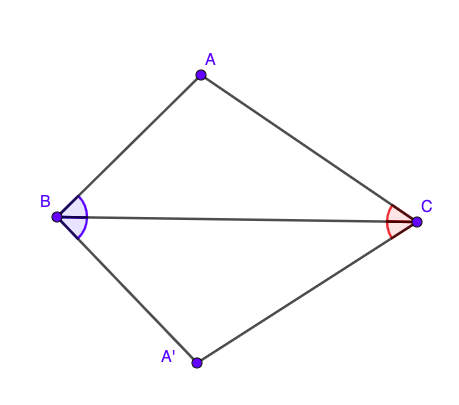
\includegraphics[scale=0.4]{iso1.png}
		\column{0.4\textwidth}
		Find an isometric transformation that maps $\triangle
		ABC$ to $\triangle A'BC$, where these two triangles
		are congruent.
	\end{columns}
\end{frame}
\begin{frame}{Isometric Transformation}
	\begin{columns}
		\column{0.6\textwidth}
		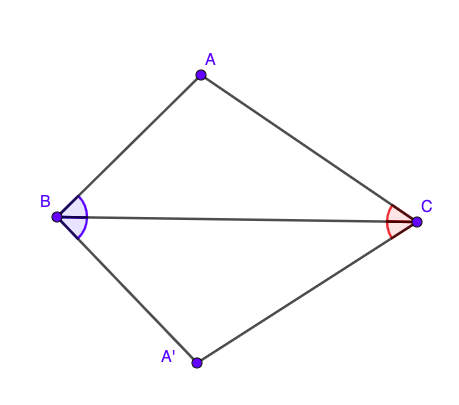
\includegraphics[scale=0.4]{iso1.png}
		\column{0.4\textwidth}
		Find an isometric transformation that maps $\triangle
		ABC$ to $\triangle A'BC$, where these two triangles
		are congruent.\\
		\phantom{Spacing}
		\textbf{Reflection} over $BC$.
	\end{columns}
\end{frame}
\begin{frame}{Isometric Transformation}
	\begin{columns}
		\column{0.6\textwidth}
		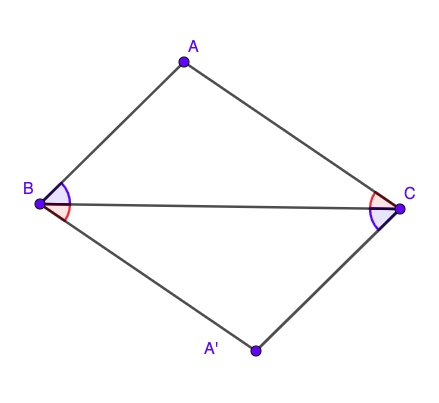
\includegraphics[scale=0.4]{iso2.png}
		\column{0.4\textwidth}
		Find an isometric transformation that maps $\triangle
		ABC$ to $\triangle A'CB$, where these two triangles
		are congruent.
	\end{columns}
\end{frame}
\begin{frame}{Isometric Transformation}
	\begin{columns}
		\column{0.6\textwidth}
		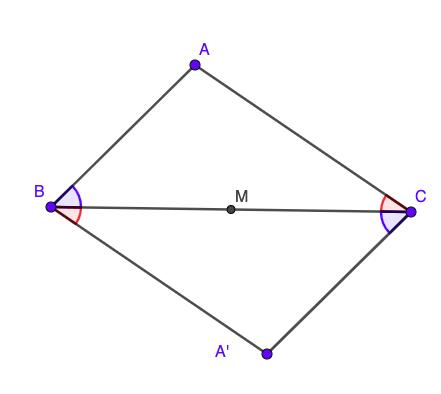
\includegraphics[scale=0.4]{iso3.png}
		\column{0.4\textwidth}
		Find an isometric transformation that maps $\triangle
		ABC$ to $\triangle A'CB$, where these two triangles
		are congruent.\\
		\phantom{Spacing}
		\textbf{Reflection} about $M$, the midpoint of $BC$.
	\end{columns}
\end{frame}
\begin{frame}{Isometric Transformation}
	\begin{columns}
		\column{0.6\textwidth}
		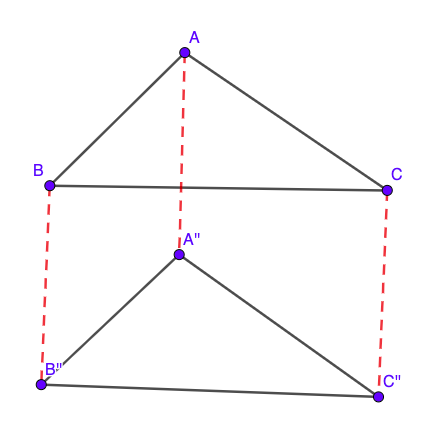
\includegraphics[scale=0.4]{iso4.png}
		\column{0.4\textwidth}
		Find an isometric transformation that maps $\triangle
		ABC$ to $\triangle A''B''C''$, where these two triangles
		are congruent. (We have 3 parallelograms.)
	\end{columns}
\end{frame}
\begin{frame}{Isometric Transformation}
	\begin{columns}
		\column{0.6\textwidth}
		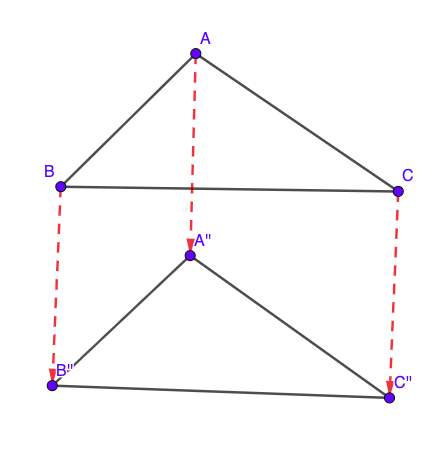
\includegraphics[scale=0.4]{iso5.png}
		\column{0.4\textwidth}
		Find an isometric transformation that maps $\triangle
		ABC$ to $\triangle A''B''C''$, where these two triangles
		are congruent. (We have 3 parallelograms.)\\
		\phantom{Spacing}
		\textbf{Translation} that takes $A$ to $A''$ (or $B$ to
		$B''$, and $C$ to $C''$).
	\end{columns}
\end{frame}
\begin{frame}{Isometric Transformation}
	\begin{columns}
		\column{0.6\textwidth}
		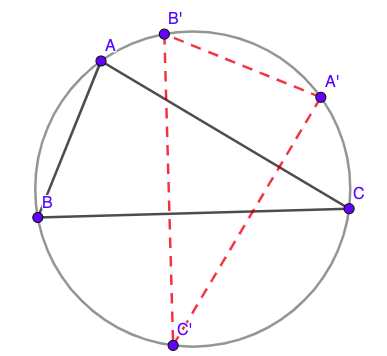
\includegraphics[scale=0.4]{iso6.png}
		\column{0.4\textwidth}
		Find an isometric transformation that maps $\triangle
		ABC$ to $\triangle A'B'C'$, where these two triangles
		are congruent. (We have all six points lie on a same
		circle.)
	\end{columns}
\end{frame}
\begin{frame}{Isometric Transformation}
	\begin{columns}
		\column{0.6\textwidth}
		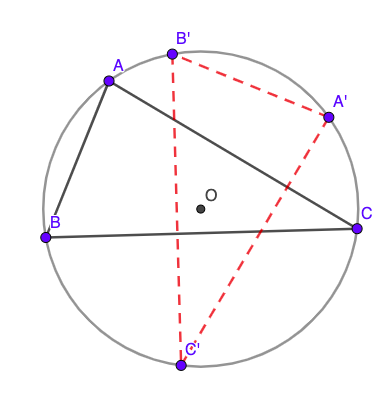
\includegraphics[scale=0.4]{iso7.png}
		\column{0.4\textwidth}
		Find an isometric transformation that maps $\triangle
		ABC$ to $\triangle A'B'C'$, where these two triangles
		are congruent. (We have all six points lie on a same
		circle.)\\
		\phantom{Spacing}
		\textbf{Rotation} about $O$, the circumcenter of 
		$\triangle ABC$.
	\end{columns}
\end{frame}
\begin{frame}{Isometric Transformation}
	\begin{columns}
		\column{0.6\textwidth}
		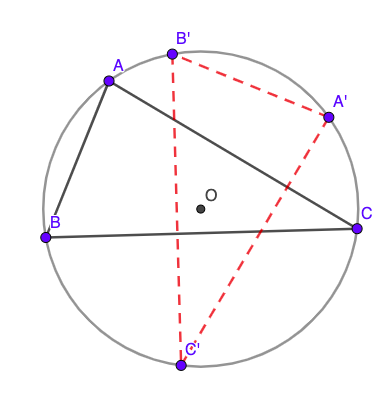
\includegraphics[scale=0.4]{iso7.png}
		\column{0.4\textwidth}
		\textbf{Rotation} about $O$, the circumcenter of 
		$\triangle ABC$.\\
		\phantom{Spacing}
		What's the rotation angle?
	\end{columns}
\end{frame}
\begin{frame}{Isometric Transformation}
	\begin{columns}
		\column{0.6\textwidth}
		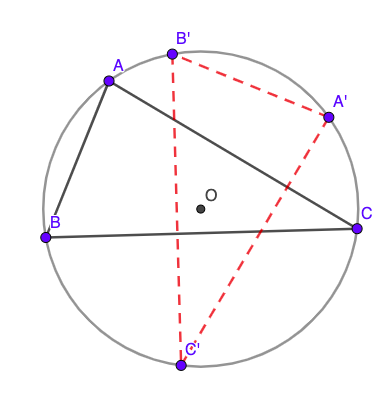
\includegraphics[scale=0.4]{iso7.png}
		\column{0.4\textwidth}
		\textbf{Rotation} about $O$, the circumcenter of 
		$\triangle ABC$.\\
		\phantom{Spacing}
		What's the rotation angle?\\
		\phantom{Spacing}
		The angle between $AB$ and $A'B'$ (or between $AC$ and
		$A'C'$, and between $BC$ and $B'C'$.)
	\end{columns}
\end{frame}
\begin{frame}{Isometric Transformations}
	\begin{columns}
		\column{0.6\textwidth}
		\includegraphics[scale=0.4]{iso8.png}
		\column{0.4\textwidth}
		What is the composition of two reflections about parallel
		lines?
	\end{columns}
\end{frame}
\begin{frame}{Isometric Transformations}
	\begin{columns}
		\column{0.6\textwidth}
		\includegraphics[scale=0.4]{iso9.png}
		\column{0.4\textwidth}
		What is the composition of two reflections about parallel
		lines?\\
		\phantom{Spacing}
		Hint: Figure.
	\end{columns}
\end{frame}
\begin{frame}{Isometric Transformations}
	\begin{columns}
		\column{0.6\textwidth}
		\includegraphics[scale=0.4]{iso10.png}
		\column{0.4\textwidth}
		What is the composition of two reflections about parallel
		lines?\\
		\phantom{Spacing}
		It is a translation.
	\end{columns}
\end{frame}
\begin{frame}{Isometric Transformations}
	\begin{columns}
		\column{0.6\textwidth}
		\includegraphics[scale=0.4]{iso10.png}
		\column{0.4\textwidth}
		What is the composition of two reflections about parallel
		lines?\\
		\phantom{Spacing}
		It is a translation.\\
		\phantom{Spacing}
		What is the distance?
	\end{columns}
\end{frame}
\begin{frame}{Isometric Transformations}
	\begin{columns}
		\column{0.6\textwidth}
		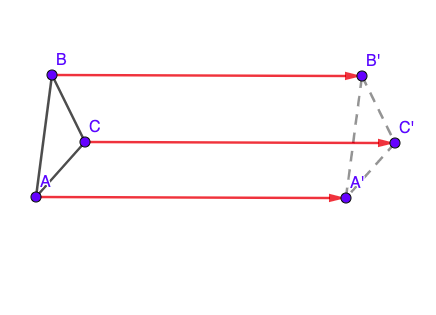
\includegraphics[scale=0.4]{iso11.png}
		\column{0.4\textwidth}
		Now, show that any translation can be written as the
		composition of two reflections.
	\end{columns}
\end{frame}
\begin{frame}{Isometric Transformations}
	\begin{columns}
		\column{0.6\textwidth}
		\includegraphics[scale=0.4]{iso10.png}
		\column{0.4\textwidth}
		Now, show that any translation can be written as the
		composition of two reflections.\\
		Take two lines that:
		\begin{itemize}
			\item are perpendicular to the translation vector
			\item have distance equal to half of the translation
				distance.
		\end{itemize}
	\end{columns}
\end{frame}
\begin{frame}{Isometric Transformations}
	\begin{columns}
		\column{0.6\textwidth}
		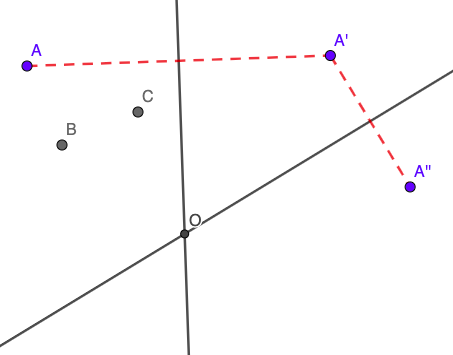
\includegraphics[scale=0.4]{iso12.png}
		\column{0.4\textwidth}
		What about the composition of two reflections with
		axes that are not parallel?
	\end{columns}
\end{frame}
\begin{frame}{Isometric Transformations}
	\begin{columns}
		\column{0.6\textwidth}
		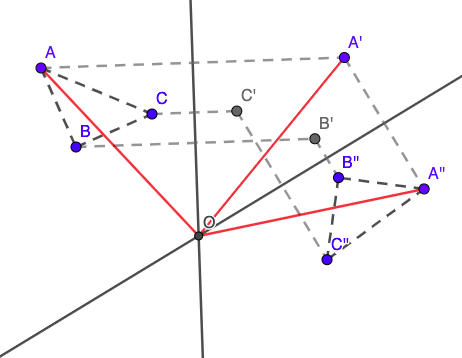
\includegraphics[scale=0.4]{iso13.png}
		\column{0.4\textwidth}
		What about the composition of two reflections with
		axes that are not parallel?\\
		\phantom{Spacing}
		\textbf{Rotation} centered at $O$, the intersection of
		two axes.
	\end{columns}
\end{frame}
\begin{frame}{Isometric Transformations}
	\begin{columns}
		\column{0.6\textwidth}
		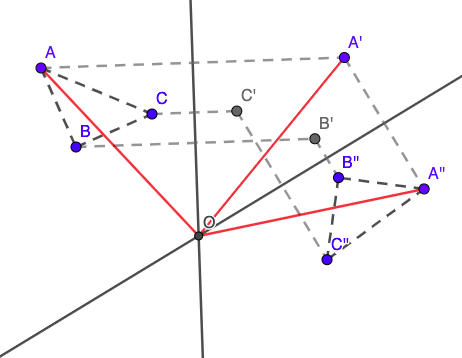
\includegraphics[scale=0.4]{iso13.png}
		\column{0.4\textwidth}
		What about the composition of two reflections with
		axes that are not parallel?\\
		\phantom{Spacing}
		\textbf{Rotation} centered at $O$, the intersection of
		two axes.\\
		\phantom{Spacing}
		What's the rotation angle?
	\end{columns}
\end{frame}
\begin{frame}{Isometric Transformations}
	\begin{columns}
		\column{0.6\textwidth}
		\includegraphics[scale=0.34]{iso23.png}
		\column{0.4\textwidth}
		$\triangle ABC$ and $\triangle A'B'C'$ have same 
		orientation, and corresponding sides are not parallel.
		Then there is a rotation that takes $\triangle ABC$ to
		$\triangle A'B'C'$.
	\end{columns}
\end{frame}
\begin{frame}{Isometric Transformations}
	\begin{columns}
		\column{0.6\textwidth}
		\includegraphics[scale=0.34]{iso23.png}
		\column{0.4\textwidth}
		$\triangle ABC$ and $\triangle A'B'C'$ have same 
		orientation, and corresponding sides are not parallel.
		Then there is a rotation that takes $\triangle ABC$ to
		$\triangle A'B'C'$.\\
		\phantom{Spacing}
		To find the center of the rotation, we can construct
		perpendicular bisectors of $A A'$ and $BB'$. Let $O$ 
		be the intersection. Then, $O$ will be the 
		center of rotation, and the rotation angle is $\angle 
		AO A'$.
	\end{columns}
\end{frame}
\begin{frame}{Isometric Transformations}
	\begin{columns}
		\column{0.6\textwidth}
		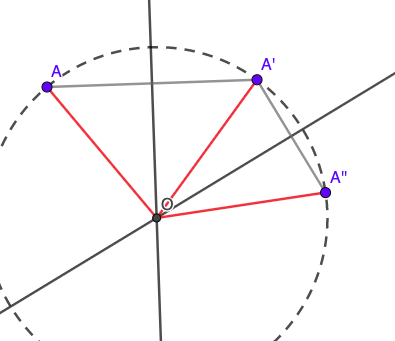
\includegraphics[scale=0.4]{iso14.png}
		\column{0.4\textwidth}
		Now, show that any rotation can be written as the 
		composition of two reflections.
	\end{columns}
\end{frame}
\begin{frame}{Isometric Transformations}
	\begin{columns}
		\column{0.6\textwidth}
		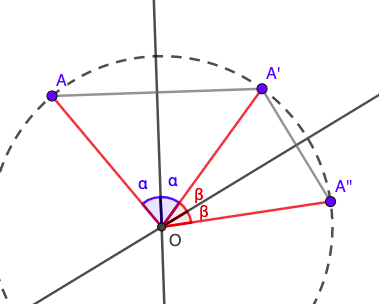
\includegraphics[scale=0.4]{iso15.png}
		\column{0.4\textwidth}
		Now, show that any rotation can be written as the 
		composition of two reflections.\\
		\phantom{Spacing}
		Take any two axes that intersect with angle that is
		half of the rotation angle.
	\end{columns}
\end{frame}
\begin{frame}{Isometric Transformations}
	\begin{columns}
		\column{0.6\textwidth}
		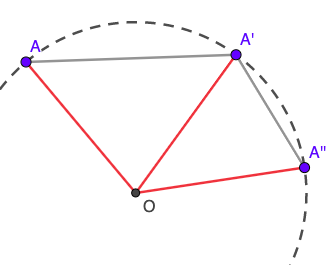
\includegraphics[scale=0.4]{iso16.png}
		\column{0.4\textwidth}
		The composition of 2 rotations with same center is a 
		rotation.
	\end{columns}
\end{frame}
\begin{frame}{Isometric Transformations}
	\begin{columns}
		\column{0.6\textwidth}
		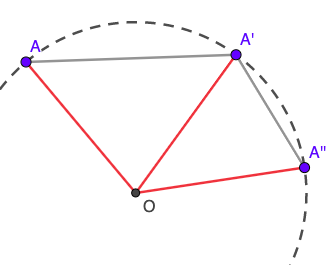
\includegraphics[scale=0.4]{iso16.png}
		\column{0.4\textwidth}
		The composition of 2 rotations with same center is a 
		rotation.\\
		\phantom{Spacing}
		Trivial.
	\end{columns}
\end{frame}
\begin{frame}{Isometric Transformations}
	\begin{columns}
		\column{0.6\textwidth}
		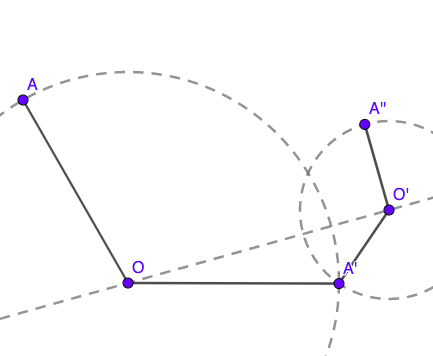
\includegraphics[scale=0.4]{iso17.png}
		\column{0.4\textwidth}
		The composition of 2 rotations with different centers
		is a translation or a rotation.
	\end{columns}
\end{frame}
\begin{frame}{Isometric Transformations}
	\begin{columns}
		\column{0.6\textwidth}
		\includegraphics[scale=0.4]{iso18.png}
		\column{0.4\textwidth}
		The composition of 2 rotations with different centers
		is a translation or a rotation.\\
		\phantom{Spacing}
		Change the rotations into 2 reflections:
		\begin{itemize}
			\item 1. $l$ and $O O'$
			\item 2. $O O'$ and $m$
		\end{itemize}
		Now this composition becomes reflection along $l$ and
		then $m$. 
	\end{columns}
\end{frame}
\begin{frame}{Isometric Transformations}
	\begin{columns}
		\column{0.6\textwidth}
		\includegraphics[scale=0.4]{iso19.png}
		\column{0.4\textwidth}
		The composition of a rotation and a translation is a
		rotation.
	\end{columns}
\end{frame}
\begin{frame}{Isometric Transformations}
	\begin{columns}
		\column{0.6\textwidth}
		\includegraphics[scale=0.4]{iso20.png}
		\column{0.4\textwidth}
		The composition of a rotation and a translation is a
		rotation.
		\phantom{Spacing}
		Change each transformation into 2 reflections:
		\begin{itemize}
			\item 1. $l$ and $m$, where $O\in m$ and 
				$m\perp A'A''$
			\item 2. $m$ and $k$
		\end{itemize}
		Now this composition becomes reflection along $l$ and
		then $k$. And their composition is a rotation.
	\end{columns}
\end{frame}
\begin{frame}{Isometric Transformations}
	\begin{columns}
		\column{0.6\textwidth}
		\includegraphics[scale=0.4]{iso21.png}
		\column{0.4\textwidth}
		The composition of three reflections with concurrent
		axes is a reflection.
	\end{columns}
\end{frame}
\begin{frame}{Isometric Transformations}
	\begin{columns}
		\column{0.6\textwidth}
		\includegraphics[scale=0.4]{iso21.png}
		\column{0.4\textwidth}
		The composition of three reflections with concurrent
		axes is a reflection.\\
		\phantom{Spacing}
		Change the first two reflections to a rotation.
		Change that rotation to two reflections, where the
		latter is the third original reflection. Now, we 
		only have one reflection.
	\end{columns}
\end{frame}
\begin{frame}{Isometric Transformations}
	\begin{columns}
		\column{0.6\textwidth}
		\includegraphics[scale=0.4]{iso22.png}
		\column{0.4\textwidth}
		The composition of three reflections with parallel axes
		is a reflection.
	\end{columns}
\end{frame}
\begin{frame}{Isometric Transformations}
	\begin{columns}
		\column{0.6\textwidth}
		\includegraphics[scale=0.4]{iso22.png}
		\column{0.4\textwidth}
		The composition of three reflections with parallel axes
		is a reflection.\\
		\phantom{Spacing}
		Change the first two reflections to a translation.
		Change the translation to two reflection, where
		the latter is the third original reflection. Now,
		we have left with only one reflection.
	\end{columns}
\end{frame}
\begin{frame}{Isometric Transformations}
	Suppose we have three reflections with axes, $l$,
	$m$, and $k$, where $l$ and $m$ are not parallel.
	We can make these transformations into three reflections 
	with axes $l'$, $m'$, and $k'$, where  $l'\parallel m'$
	and $m'\perp k'$ (this is called a glide reflection.)
\end{frame}
\begin{frame}{Isometric Transformations}
	\[
		(l, m, k) \to (l', m', k'), l'\parallel m', m'\perp k'
	.\] 
\end{frame}
\begin{frame}{Isometric Transformations}
	\[
		(l, m, k) \to (l', m', k'), l'\parallel m', m'\perp k'
	.\] 
	Change $(l, m) \to$ a rotation, $r$. \\

	So, $(l, m, k) \to (r, k)$
\end{frame}
\begin{frame}{Isometric Transformations}
	\[
		(r, k) \to (l', m', k'), l'\parallel m', m'\perp k'
	.\] 
	Change $r\to (l'', m'')$, where $m''\perp k$.\\

	So, $(r, k)\to (l'', m'', k)$ where $m''\perp k$.
\end{frame}
\begin{frame}{Isometric Transformations}
	\[
		(l'', m'', k), m''\perp k 
		\to (l', m', k'), l'\parallel m', m'\perp k'
	.\] 
	Change $(m'', k) \to$ a rotation, $r'$.\\

	So, $(l'', m'', k) \to (l'', r')$.
\end{frame}
\begin{frame}{Isometric Transformations}
	\[
		(l'',r')
		\to (l', m', k'), l'\parallel m', m'\perp k'
	.\] 
	Change $r'\to (m', k')$, where $m'\parallel l''$.\\

	So, $(l'', r')\to  (l'', m', k')$, where $l''\parallel m'$.\\

	And we know that $m'\perp k'$.
\end{frame}
\begin{frame}{Isometric Transformations}
	\[
		(l'',m', k'), l''\parallel m', m'\perp k'
		\to (l', m', k'), l'\parallel m', m'\perp k'
	.\] 
	Take $l'$ as $l''$. Now, we are done.
\end{frame}
\begin{frame}{Isometric Transformations}
	Suppose we have three reflections with axes, $l$, $m$, and $k$,
	where $l$ and $m$ are parallel. We can can these transformations
	into three reflections with axes $l'$, $m'$, and $k'$, which 
	results a glide reflections, i.e. $l'\parallel m'$ and $m'\perp k'$.
\end{frame}
\begin{frame}{Isometric Transformations}
	\[
		(l, m, k)\to (l', m', k'), l' \parallel m', m'\perp k'
	.\] 
\end{frame}
\begin{frame}{Isometric Transformations}
	\[
		(l, m, k)\to (l', m', k'), l' \parallel m', m'\perp k'
	.\] 
	Change $(m, k)\to$ a rotation $r$.\\

	So, $(l,m, k)\to (l, r)$.
\end{frame}
\begin{frame}{Isometric Transformations}
	\[
		(l,r)\to (l', m', k'), l' \parallel m', m'\perp k'
	.\] 
	Change $r\to (m'', k'')$ where  $m''$ is not parallel to $l$.\\

	So, $(l, r)\to (l, m'', k'')$, which is the first case we have
	considered.
\end{frame}
\begin{frame}{Isometric Transformations}
	\large{\textbf{Main Theorem}}:
	Suppose we have a isometric transformation that is a composition
	of translation, rotation, and reflection. Then, this isometric
	transformation can be reduced to no more than three reflections.
\end{frame}
\begin{frame}{Isometric Transformations}
	\large{\textbf{Main Theorem}}:
	Suppose we have a isometric transformation that is a composition
	of translation, rotation, and reflection. Then, this isometric
	transformation can be reduced to no more than three reflections.\\

	E.g. The composition can be:
	\begin{itemize}
		\item $Re_1 Re_2 T_1 Ro_1 Ro_1 T_2 T_3$
		\item $T_1 T_2 T_3 T_4$
		\item etc.
	\end{itemize}
\end{frame}
\begin{frame}{Isometric Transformations}
	\large{\textbf{Main Theorem}}:
	Suppose we have a isometric transformation that is a composition
	of translation, rotation, and reflection. Then, this isometric
	transformation can be reduced to no more than three reflections.\\

	E.g. The composition can be:
	\begin{itemize}
		\item $Re_1 Re_2 T_1 Ro_1 Ro_1 T_2 T_3$
		\item $T_1 T_2 T_3 T_4$
		\item etc.
	\end{itemize}
	\textbf{Proof}.\\
	Use previous results, and then a little combinatorics problem? :)
\end{frame}
\begin{frame}{Isometric Transformations}
	\begin{columns}
		\column{0.6\textwidth}
		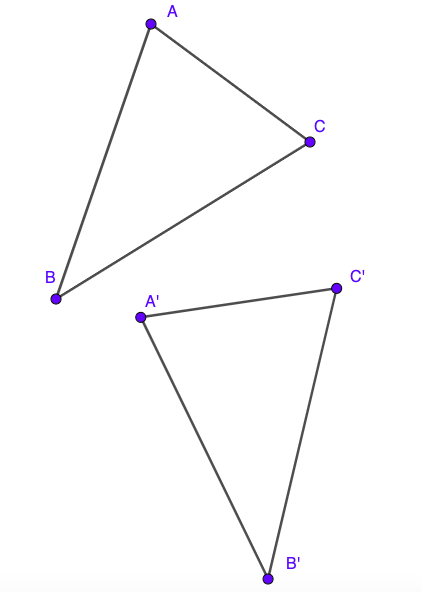
\includegraphics[scale=0.3]{cong1.png}
		\column{0.4\textwidth}
		Suppose we have two congruent triangles. Show that 
		we can find a composition that is no more than 
		three reflections that maps $\triangle ABC\to \triangle
		A'B'C'$
	\end{columns}
\end{frame}
\begin{frame}{Isometric Transformations}
	\begin{columns}
		\column{0.6\textwidth}
		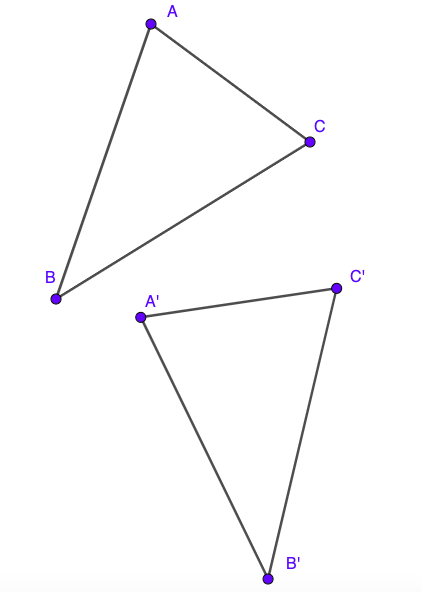
\includegraphics[scale=0.3]{cong1.png}
		\column{0.4\textwidth}
		Suppose we have two congruent triangles. Show that 
		we can find a composition that is no more than 
		three reflections that maps $\triangle ABC\to \triangle
		A'B'C'$\\
		\phantom{Spacing}
		\textbf{Hint}: Take midpoint of $A A'$, $BB'$, and $C C'$.
		They will tell you what kind of transformations we need.
	\end{columns}
\end{frame}

\begin{frame}{Spiral Similarity}
	\begin{columns}
		\column{0.6\textwidth}
		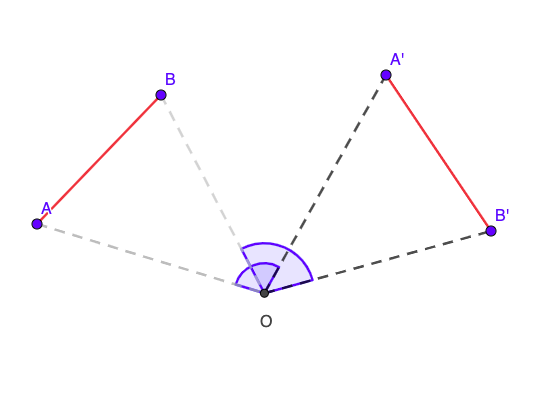
\includegraphics[scale=0.34]{spi1.png}
		\column{0.4\textwidth}
		$Scale$ and $rotate$ with given center $O$ and angle
		$\alpha$ and scale factor $k$.
	\end{columns}
\end{frame}
\begin{frame}{Spiral Similarity}
	\begin{columns}
		\column{0.6\textwidth}
		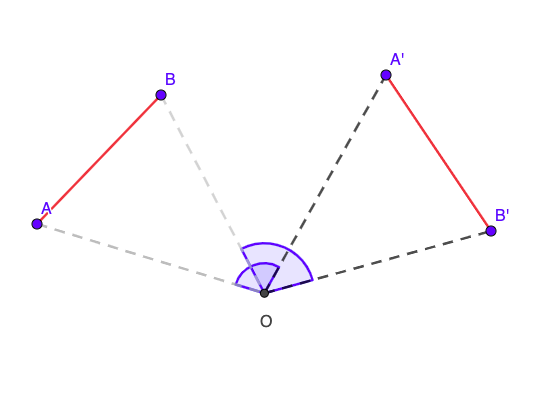
\includegraphics[scale=0.34]{spi1.png}
		\column{0.4\textwidth}
		$Scale$ and $rotate$ with given center $O$ and angle
		$\alpha$ and scale factor $k$:
		\begin{itemize}
			\item $OA' = kOA$
			\item $\angle AOA' = \alpha$
			\item $OB' = kOB$
			\item $\angle BOB' = \alpha$
		\end{itemize}
	\end{columns}
\end{frame}
\begin{frame}{Spiral Similarity}
	\begin{columns}
		\column{0.6\textwidth}
		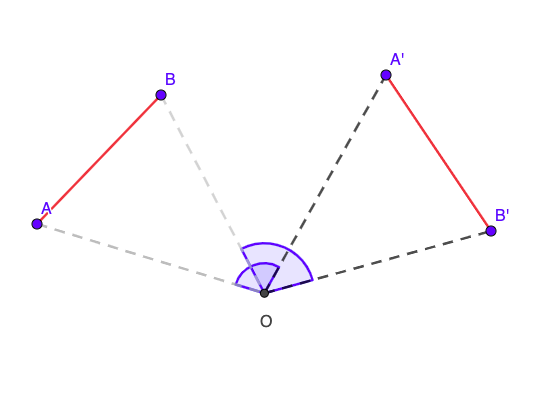
\includegraphics[scale=0.4]{spi1.png}
		\column{0.4\textwidth}
		$Scale$ and $rotate$ with given center $O$ and angle
		$\alpha$ and scale factor $k$:
		\begin{itemize}
			\item $OA' = kOA$
			\item $\angle AOA' = \alpha$
			\item $OB' = kOB$
			\item $\angle BOB' = \alpha$
		\end{itemize}
		As a consequence, $A'B' = kAB$.
	\end{columns}
\end{frame}
\begin{frame}{Spiral Similarity}
	\begin{columns}
		\column{0.6\textwidth}
		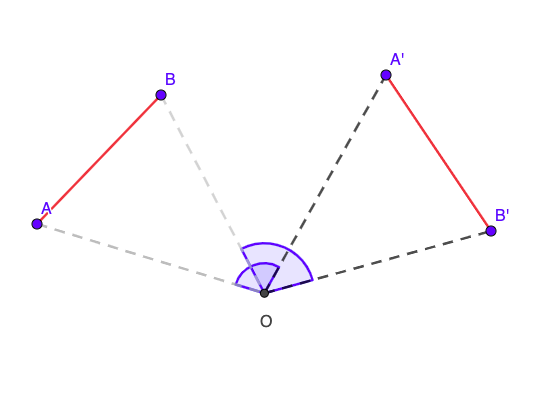
\includegraphics[scale=0.4]{spi1.png}
		\column{0.4\textwidth}
		$Scale$ and $rotate$ with given center $O$ and angle
		$\alpha$ and scale factor $k$:
		\begin{itemize}
			\item $OA' = kOA$
			\item $\angle AOA' = \alpha$
			\item $OB' = kOB$
			\item $\angle BOB' = \alpha$
		\end{itemize}
		As a consequence, $A'B' = kAB$.\\
		Also, $OA\cdot OB' = OB\cdot OA'$.
	\end{columns}
\end{frame}
\begin{frame}{Spiral Similarity}
	\begin{columns}
		\column{0.6\textwidth}
		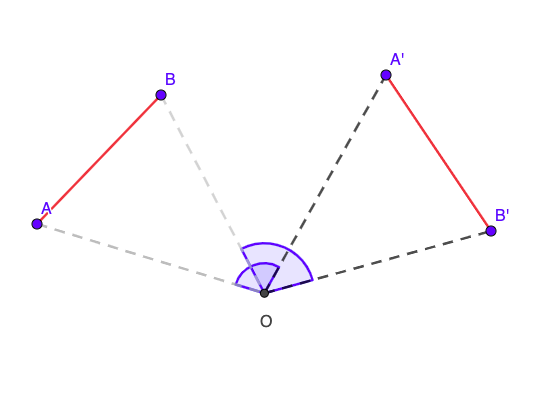
\includegraphics[scale=0.37]{spi1.png}
		\column{0.4\textwidth}
		Suppose we don't know the spiral similarity center 
		but only know $A$ and $B$ goes to $A'$ and $B'$.\\
		\phantom{Spacing}
		How do we find the center?
	\end{columns}
\end{frame}
\begin{frame}{Spiral Similarity}
	\begin{columns}
		\column{0.6\textwidth}
		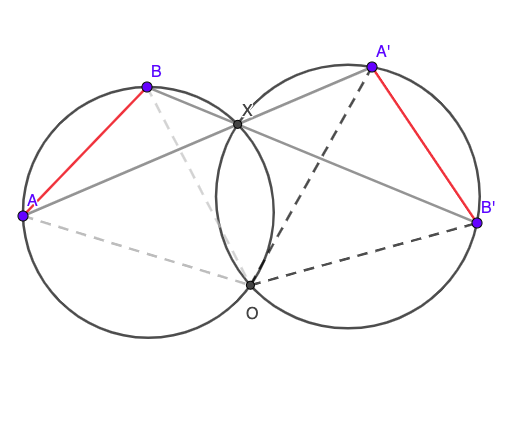
\includegraphics[scale=0.37]{spi2.png}
		\column{0.4\textwidth}
		How do we find the center?\\
		\phantom{Spacing}
		$X = A A'\cap BB'$ \\
		$O = \omega(ABX) \cap \omega(A'B'X')$.
	\end{columns}
\end{frame}
\begin{frame}{Spiral Similarity}
	\begin{columns}
		\column{0.6\textwidth}
		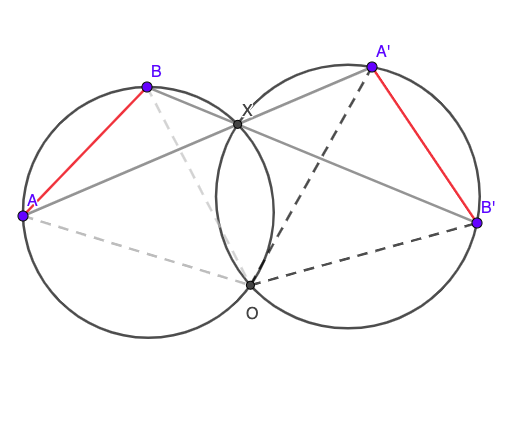
\includegraphics[scale=0.37]{spi2.png}
		\column{0.4\textwidth}
		$X = A A'\cap BB'$ \\
		$O = \omega(ABX) \cap \omega(A'B'X')$.\\
		\phantom{Spacing}
		Show that $O$ is the center of the spiral similarity.
	\end{columns}
\end{frame}
\begin{frame}{Spiral Similarity}
	\begin{columns}
		\column{0.6\textwidth}
		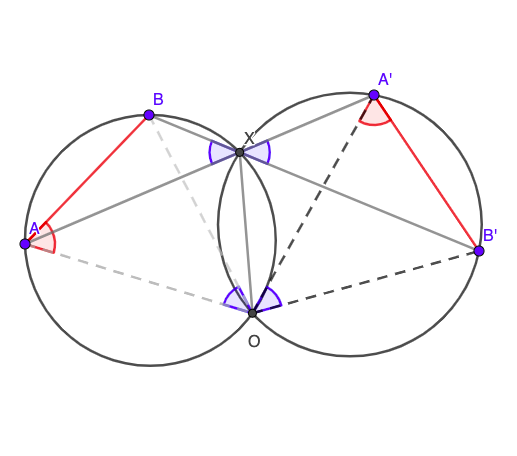
\includegraphics[scale=0.37]{spi3.png}
		\column{0.4\textwidth}
		Show that $O$ is the center of the spiral similarity.\\
		\phantom{Spacing}
		In other words, we just need to show $\triangle AOB\sim
		\triangle A'OB'$.
	\end{columns}
\end{frame}
\begin{frame}{Spiral Similarity}
	\begin{columns}
		\column{0.6\textwidth}
		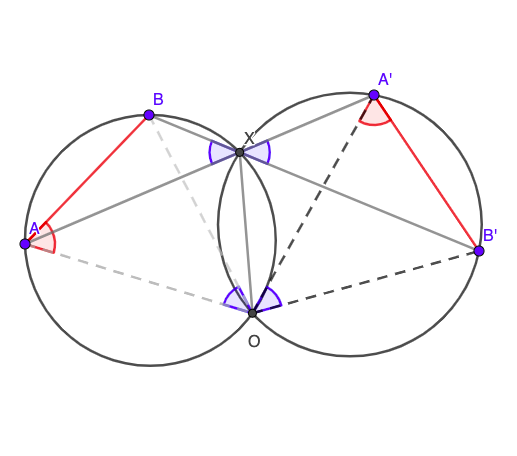
\includegraphics[scale=0.37]{spi3.png}
		\column{0.4\textwidth}
		Show that $O$ is the center of the spiral similarity.\\
		\phantom{Spacing}
		In other words, we just need to show $\triangle AOB\sim
		\triangle A'OB'$. This is true by AA. 
	\end{columns}
\end{frame}
\begin{frame}{Spiral Similarity}
	\begin{columns}
		\column{0.6\textwidth}
		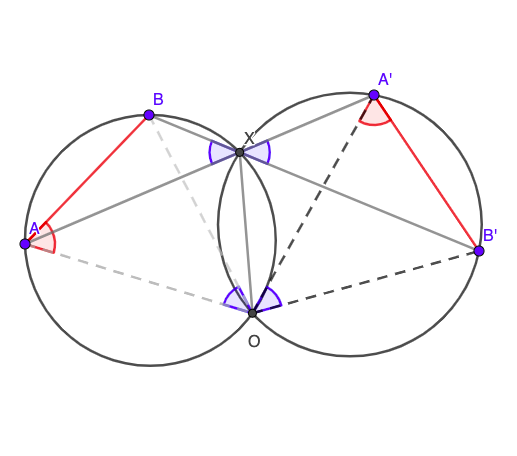
\includegraphics[scale=0.37]{spi3.png}
		\column{0.4\textwidth}
		Suppose a spiral similarity centered at $O$ takes
		$AB$ to $A'B'$. Then, show that there is a spiral 
		similarity centered at $O$ takes $A A'$ to $BB'$.
	\end{columns}
\end{frame}
\begin{frame}{Spiral Similarity}
	\begin{columns}
		\column{0.6\textwidth}
		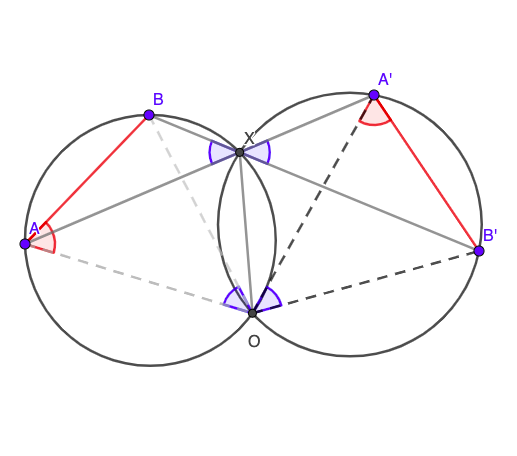
\includegraphics[scale=0.37]{spi3.png}
		\column{0.4\textwidth}
		Suppose a spiral similarity centered at $O$ takes
		$AB$ to $A'B'$. Then, show that there is a spiral 
		similarity centered at $O$ takes $A A'$ to $BB'$.\\
		\phantom{Spacing}
		We just need to show $\triangle OA A'\sim \triangle OBB'$.
	\end{columns}
\end{frame}
\begin{frame}{Spiral Similarity}
	\begin{columns}
		\column{0.6\textwidth}
		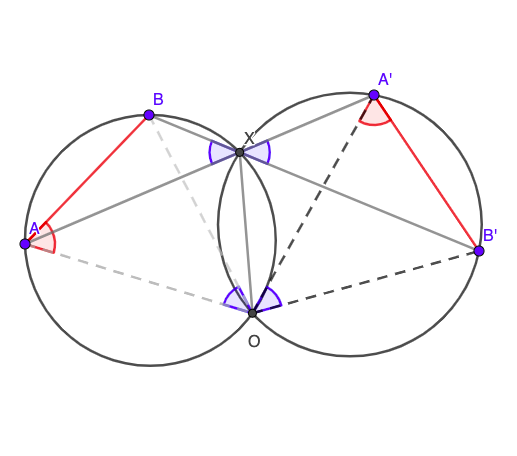
\includegraphics[scale=0.37]{spi3.png}
		\column{0.4\textwidth}
		Suppose a spiral similarity centered at $O$ takes
		$AB$ to $A'B'$. Then, show that there is a spiral 
		similarity centered at $O$ takes $A A'$ to $BB'$.\\
		\phantom{Spacing}
		We just need to show $\triangle OA A'\sim \triangle OBB'$:
		\begin{itemize}
			\item $\angle AOA' = \angle BOB'$
			\item $\frac{OA}{OB} = \frac{kOA}{kOB} = \frac{OA'}{OB'}$
		\end{itemize}
	\end{columns}
\end{frame}
\begin{frame}{Spiral Similarity}
	\begin{columns}
		\column{0.6\textwidth}
		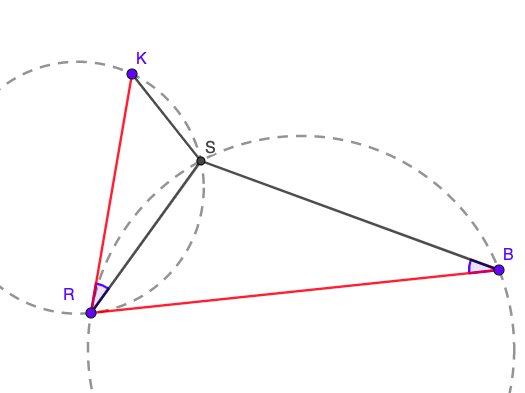
\includegraphics[scale=0.34]{spi4.png}
		\column{0.4\textwidth}
		Consider spiral similarity centered at $S$ that takes
		$KR$ to $RB$. What can we tell about this situation?
	\end{columns}
\end{frame}
\begin{frame}{Spiral Similarity}
	\begin{columns}
		\column{0.6\textwidth}
		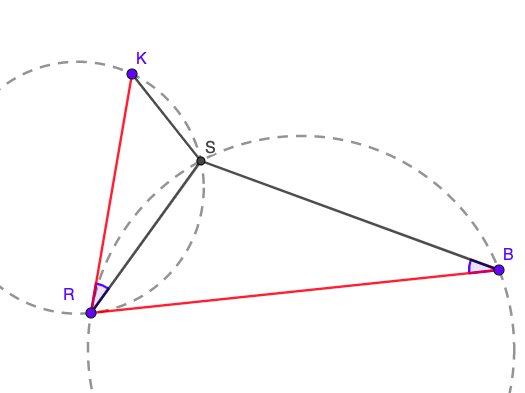
\includegraphics[scale=0.34]{spi4.png}
		\column{0.4\textwidth}
		Consider spiral similarity centered at $S$ that takes
		$KR$ to $RB$. What can we tell about this situation?\\
		\phantom{Spacing}
		We can deduce that $KR$ is tangent to $\omega(SRB)$.\\
		Similarly, $RB$ is tangent to $\omega(SKR)$.
	\end{columns}
\end{frame}
\begin{frame}{Spiral Similarity}
	\begin{columns}
		\column{0.6\textwidth}
		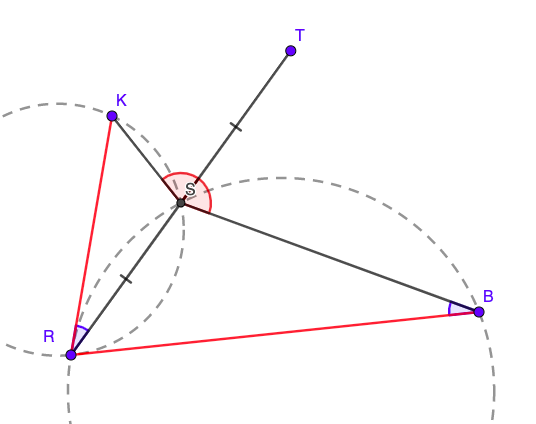
\includegraphics[scale=0.34]{spi5.png}
		\column{0.4\textwidth}
		Consider spiral similarity centered at $S$ that takes
		$KR$ to $RB$. What can we tell about this situation?\\
		$RB$ is tangent to $\omega(SKR)$.\\
		\phantom{Spacing}
		Now, construct $T$ such that $RS = ST$ and $T\in RS$.
		In other words, $T$ is the reflection of $R$ about $S$.
	\end{columns}
\end{frame}
\begin{frame}{Spiral Similarity}
	\begin{columns}
		\column{0.6\textwidth}
		\includegraphics[scale=0.34]{spi5.png}
		\column{0.4\textwidth}
		$S$ takes $KR$ to $RB$.\\
		$RB$ is tangent to $\omega(SKR)$.\\
		\phantom{Spacing}
		$T$ is the reflection of $R$ about $S$. Can we say 
		$S$ takes $KT$ to $TB$?
	\end{columns}
\end{frame}
\begin{frame}{Spiral Similarity}
	\begin{columns}
		\column{0.6\textwidth}
		\includegraphics[scale=0.34]{spi5.png}
		\column{0.4\textwidth}
		$T$ is the reflection of $R$ about $S$. Can we say 
		$S$ takes $KT$ to $TB$?\\
		\phantom{Spacing}
		Yes:
		\begin{itemize}
			\item $\frac{KS}{ST} = \frac{KS}{SR} = \frac{RS}{
				SB} = \frac{TS}{SB}$
			\item $\angle KST = \angle BST$
		\end{itemize}
	\end{columns}
\end{frame}
\begin{frame}{Spiral Similarity}
	\begin{columns}
		\column{0.6\textwidth}
		\includegraphics[scale=0.34]{spi5.png}
		\column{0.4\textwidth}
		So, $S$ takes $KT$ to $TB$.\\
	\end{columns}
\end{frame}
\begin{frame}{Spiral Similarity}
	\begin{columns}
		\column{0.6\textwidth}
		\includegraphics[scale=0.34]{spi5.png}
		\column{0.4\textwidth}
		So, $S$ takes $KT$ to $TB$.\\
		\phantom{Spacing}
		Now, what do we know about in this scenario?
	\end{columns}
\end{frame}
\begin{frame}{Spiral Similarity}
	\begin{columns}
		\column{0.6\textwidth}
		\includegraphics[scale=0.34]{spi5.png}
		\column{0.4\textwidth}
		So, $S$ takes $KT$ to $TB$.\\
		\phantom{Spacing}
		Now, what do we know about in this scenario?\\
		\phantom{Spacing}
		We know that $KT$ is tangent to $\omega(STB)$.
	\end{columns}
\end{frame}
\begin{frame}{Moving to P4, IMO 2017}
	\begin{columns}
		\column{0.6\textwidth}
		\includegraphics[scale=0.46]{spi6.png}
		\column{0.4\textwidth}
		\small{
		Let $R$ and $S$ be distinct points on circle $\Omega$,
		and let $t$ denote the tangent line to $\Omega$ at $R$.
		Point $T$ is the reflection of $R$ with respect to $S$.
		A point $I$ is chosen on the smaller arc $RS$ of 
		$\Omega$ so that the circumcircle $\Gamma$ of triangle
		$IST$ intersect $t$ at two different points. Denote by
		$A$ the common point of $\Gamma$ and $t$ that is closest
		to $R$. Line $AI$ meets $\Omega$ again at $K$. Show that
		$KT$ is tangent to $\Gamma$.
		}
	\end{columns}
\end{frame}
\begin{frame}{Moving to IMO 2017 P4}
	\begin{columns}
		\column{0.6\textwidth}
		\includegraphics[scale=0.46]{spi6.png}
		\column{0.4\textwidth}
		Show that $KT$ is tangent to $\Gamma$.\\
		\phantom{Spacing}
		We just need to see $S$ takes $KR$ to $RB$. Then, we are
		done \Laughey
	\end{columns}
\end{frame}
\begin{frame}{Spiral Similarity}
	\begin{columns}
		\column{0.6\textwidth}
		\includegraphics[scale=0.34]{spi7.png}
		\column{0.4\textwidth}
		$\triangle ABC$, $AB >  BC$,\\ 
		$D\in BC$, $E\in \omega(ABC)$,\\
		$\angle BAE = \angle DAC$.\\
		\phantom{Spacing}
		Show that a spiral similarity centered at $A$ takes
		$BD$ to $EC$.
	\end{columns}
\end{frame}
\begin{frame}{Spiral Similarity}
	\begin{columns}
		\column{0.6\textwidth}
		\includegraphics[scale=0.34]{spi8.png}
		\column{0.4\textwidth}
		Show that a spiral similarity centered at $A$ takes
		$BD$ to $EC$.\\
		\phantom{Spacing}
		By AA:
		\begin{itemize}
			\item $\angle BAD = \angle EAC$
			\item $\angle ABD = \angle AEC$
		\end{itemize}
	\end{columns}
\end{frame}
\begin{frame}{Spiral Similarity}
	\begin{columns}
		\column{0.6\textwidth}
		\includegraphics[scale=0.34]{spi9.png}
		\column{0.4\textwidth}
		$\triangle ABD \sim \triangle AEC$\\
		$I$ - incenter of $\triangle ABD$\\
		$J$ - incenter of $\triangle AEC$.\\
		\phantom{Spacing}
		Show that a spiral similarity centered at $A$ takes
		$DI$ to $CJ$.
	\end{columns}
\end{frame}
\begin{frame}{Spiral Similarity}
	\begin{columns}
		\column{0.6\textwidth}
		\includegraphics[scale=0.34]{spi9.png}
		\column{0.4\textwidth}
		Show that a spiral similarity centered at $A$ takes
		$ID$ to $JC$.\\
		\phantom{Spacing}
		Since $\triangle ABD\sim \triangle AEC$, we have
		$\triangle AID\sim \triangle BJC$ by AA:
		\begin{itemize}
			\item $\angle AID = 90^\circ \beta / 2 = \angle AJC$
			\item $\angle IAD = \angle BAD / 2 = \angle EAC / 2
				= \angle JAC$
		\end{itemize}
	\end{columns}
\end{frame}
\begin{frame}{Spiral Similarity}
	\begin{columns}
		\column{0.6\textwidth}
		\includegraphics[scale=0.34]{spi10.png}
		\column{0.4\textwidth}
		A spiral similarity centered at $A$ takes $ID$ to $JC$.\\
		$Q = IJ\cap BC$.\\
		\phantom{Spacing}
		Where are the two cyclic quadrilaterals we have?
	\end{columns}
\end{frame}
\begin{frame}{Spiral Similarity}
	\begin{columns}
		\column{0.6\textwidth}
		\includegraphics[scale=0.34]{spi11.png}
		\column{0.4\textwidth}
		A spiral similarity centered at $A$ takes $ID$ to $JC$.\\
		$Q = IJ\cap BC$.\\
		\phantom{Spacing}
		Where are the two cyclic quadrilaterals we have?\\
		\phantom{Spacing}
		The quadrilaterals $AIDQ$ and $AJCQ$ are cyclic.
	\end{columns}
\end{frame}
\begin{frame}{Moving to P3, CMC 2020}
	\begin{columns}
		\column{0.6\textwidth}
		\includegraphics[scale=0.34]{spi11.png}
		\column{0.4\textwidth}
		\small{
		Let $ABC$ be a triangle such that $AB>BC$ and let $D$ 
		be a variable point on the line segment $BC$. Let $ E$
		be a point on the circumcircle of triangle $ABC$, lying
		on the opposite side of $BC$ from $A$ such that 
		$\angle BAE = \angle DAC$. Let $I$ be the incenter of 
		triangle $ABD$ and let $J$ be the incenter of triangle $
		ACE$. Prove that the line $IJ$ passes through a fixed
		point, that is independent of $D$.
		}
	\end{columns}
\end{frame}
\begin{frame}{Moving to P3, CMC 2020}
	\begin{columns}
		\column{0.6\textwidth}
		\includegraphics[scale=0.34]{spi11.png}
		\column{0.4\textwidth}
		Prove that the line $IJ$ passes through a fixed
		point, that is independent of $D$.\\
		\phantom{Spacing}
		We claim that the independent point that the problem is
		referring is indeed $Q$.
	\end{columns}
\end{frame}
\begin{frame}{Moving to P3, CMC 2020}
	\begin{columns}
		\column{0.6\textwidth}
		\includegraphics[scale=0.34]{spi11.png}
		\column{0.4\textwidth}
		We claim that the independent point that the problem is
		referring is indeed $Q$. In other words, no matter
		how we move $D$ along $BC$, $Q$ will be in same position.
	\end{columns}
\end{frame}
\begin{frame}{Moving to P3, CMC 2020}
	\begin{columns}
		\column{0.6\textwidth}
		\includegraphics[scale=0.34]{spi11.png}
		\column{0.4\textwidth}
		In other words, no matter
		how we move $D$ along $BC$, $Q$ will be in same position.\\
		\phantom{Spacing}
		Why?
	\end{columns}
\end{frame}
\begin{frame}{Moving to P3, CMC 2020}
	\begin{columns}
		\column{0.6\textwidth}
		\includegraphics[scale=0.34]{spi11.png}
		\column{0.4\textwidth}
		In other words, no matter
		how we move $D$ along $BC$, $Q$ will be in same position.\\
		\phantom{Spacing}
		Why?\\
		\phantom{Spacing}
		Take a point, $Q'$, on $BC$ such that $\angle AQ'C = 
		90^\circ - \beta/2$. We know that $Q'$ is independent of $D$
		.
	\end{columns}
\end{frame}
\begin{frame}{Moving to P3, CMC 2020}
	\begin{columns}
		\column{0.6\textwidth}
		\includegraphics[scale=0.34]{spi11.png}
		\column{0.4\textwidth}
		Take a point, $Q'$, on $BC$ such that $\angle AQ'C = 
		90^\circ - \beta/2$. We know that $Q'$ is independent of $D$
		.\\
		\phantom{Spacing}
		Now, consider $\angle AQC$.
	\end{columns}
\end{frame}
\begin{frame}{Moving to P3, CMC 2020}
	\begin{columns}
		\column{0.6\textwidth}
		\includegraphics[scale=0.34]{spi11.png}
		\column{0.4\textwidth}
		Take a point, $Q'$, on $BC$ such that $\angle AQ'C = 
		90^\circ - \beta/2$. We know that $Q'$ is independent of $D$
		.\\
		\phantom{Spacing}
		$\angle AQC = 180^\circ - \angle AJC = 180^\circ - 
		(90^\circ + \beta /  2) = 90^\circ - \beta / 2$.
	\end{columns}
\end{frame}
\begin{frame}{Moving to P3, CMC 2020}
	\begin{columns}
		\column{0.6\textwidth}
		\includegraphics[scale=0.34]{spi11.png}
		\column{0.4\textwidth}
		Take a point, $Q'$, on $BC$ such that $\angle AQ'C = 
		90^\circ - \beta/2$. We know that $Q'$ is independent of $D$
		.\\
		Hence, $Q$ is $Q'$, meaning $Q$ is independent of $D$.
	\end{columns}
\end{frame}

\begin{frame}{Back to Power of Point}
	\begin{columns}
		\column{0.6\textwidth}
		\includegraphics[scale=0.4]{pip1.png}
		\column{0.4\textwidth}
		We define power of a point $P$ with respect to circle
		$\omega$ as:
		\[
			Pow(P, \omega) = PA\cdot PB
		.\] 
	\end{columns}
\end{frame}
\begin{frame}{Back to Power of Point}
	\begin{columns}
		\column{0.6\textwidth}
		\includegraphics[scale=0.4]{pip1.png}
		\column{0.4\textwidth}
		This is also equal to
		\[
			Pow(P, \omega) = PC^2
		.\] 
	\end{columns}
\end{frame}
\begin{frame}{Back to Power of Point}
	\begin{columns}
		\column{0.6\textwidth}
		\includegraphics[scale=0.4]{pip1.png}
		\column{0.4\textwidth}
		And
		\[
			Pow(P, \omega) = PO^2 - r^2
		,\] where $r$ is the radius of $\omega$.
	\end{columns}
\end{frame}

\begin{frame}{Radical Axis}
	\begin{columns}
		\column{0.6\textwidth}
		\includegraphics[scale=0.4]{rad1.png}
		\column{0.4\textwidth}
		$Pow(P, \omega) = PO^2 - r^2$.\\
		\phantom{Spacing}
		Suppose, we have two circles, $\omega_1$ and $\omega_2$.
	\end{columns}
\end{frame}
\begin{frame}{Radical Axis}
	\begin{columns}
		\column{0.6\textwidth}
		\includegraphics[scale=0.4]{rad1.png}
		\column{0.5\textwidth}
		Suppose, we have two circles, $\omega_1$ and $\omega_2$.\\
		We want to consider a set of points whose powers
		to these circles are equal:
		\[
			\{ P | Pow(P, \omega_1) = Pow(P,\omega_2)\}
		.\] 
	\end{columns}
\end{frame}
\begin{frame}{Radical Axis}
	\begin{columns}
		\column{0.6\textwidth}
		\includegraphics[scale=0.4]{rad1.png}
		\column{0.5\textwidth}
		We claim that this set forms a line.
		\[
			\{ P | Pow(P, \omega_1) = Pow(P,\omega_2)\}
		.\] 
	\end{columns}
\end{frame}
\begin{frame}{Radical Axis}
	\begin{columns}
		\column{0.6\textwidth}
		\includegraphics[scale=0.4]{rad1.png}
		\column{0.5\textwidth}
		$P = (x,y)$ \\
		$O_1 = (a, b)$\\
		$O_2 = (c, d)$.\\
		\phantom{Spacing}
		We have, \\
		$
			(x-a)^2 + (y-b)^2 - r_1^2 = (x-c)^2 + (y-d)^2 - r_2^2
			.$
	\end{columns}
\end{frame}
\begin{frame}{Radical Axis}
	\begin{columns}
		\column{0.6\textwidth}
		\includegraphics[scale=0.4]{rad1.png}
		\column{0.4\textwidth}
		$P = (x,y)$ \\
		$O_1 = (a, b)$\\
		$O_2 = (c, d)$.\\
		\phantom{Spacing}
		After cancelling $x^2$ and $y^2$, we have:
		\[
			mx + ny +p = 0
		,\] which is the equation of line.
	\end{columns}
\end{frame}
\begin{frame}{Radical Axis}
	\begin{columns}
		\column{0.6\textwidth}
		\includegraphics[scale=0.4]{rad1.png}
		\column{0.4\textwidth}
		Now, this line is called the radical axis of the circles
		$\omega_1$ and $\omega_2$.
	\end{columns}
\end{frame}
\begin{frame}{Radical Axis}
	\begin{columns}
		\column{0.6\textwidth}
		\includegraphics[scale=0.4]{rad1.png}
		\column{0.4\textwidth}
		If $\omega_1$ and $\omega_2$ intersects, then 
		the common chord is the radical axis.\\
		\phantom{Spacing}
		Why?
	\end{columns}
\end{frame}
\begin{frame}{Radical Axis}
	\begin{columns}
		\column{0.6\textwidth}
		\includegraphics[scale=0.4]{rad1.png}
		\column{0.4\textwidth}
		If $\omega_1$ and $\omega_2$ intersects, then 
		the common chord is the radical axis since
		the powers of the intersections points are zero.
	\end{columns}
\end{frame}
\begin{frame}{Radical Axis}
	\begin{columns}
		\column{0.6\textwidth}
		\includegraphics[scale=0.23]{rad5.png}
		\column{0.4\textwidth}
		$\omega_1$ and $\omega_2$ does not intersect.
	\end{columns}
\end{frame}
\begin{frame}{Radical Axis}
	\begin{columns}
		\column{0.6\textwidth}
		\includegraphics[scale=0.4]{rad2.png}
		\column{0.4\textwidth}
		$\omega_1$ and $\omega_2$ intersects at $AB$.
		$MN$ is the common tangent.\\
		\phantom{Spacing}
		Show that $AB$ bisects the segment $MN$.
	\end{columns}
\end{frame}
\begin{frame}{Radical Axis}
	\begin{columns}
		\column{0.6\textwidth}
		\includegraphics[scale=0.4]{rad3.png}
		\column{0.4\textwidth}
		Show that $AB$ bisects the segment $MN$.\\
		\phantom{Spacing}
		Let $P$ be the intersection of $AB$ and $MN$.\\
		We know that $AB$ is the radical axis.\\
		So, $Pow(P, \omega_1) = Pow(P, \omega_2)$.
	\end{columns}
\end{frame}
\begin{frame}{Radical Axis}
	\begin{columns}
		\column{0.6\textwidth}
		\includegraphics[scale=0.4]{rad3.png}
		\column{0.4\textwidth}
		Show that $AB$ bisects the segment $MN$.\\
		\phantom{Spacing}
		Let $P$ be the intersection of $AB$ and $MN$.\\
		We know that $AB$ is the radical axis.\\
		So, $Pow(P, \omega_1) = Pow(P, \omega_2)$.\\
		\phantom{Spacing}
		But what is $Pow(P,\omega_1)$?
	\end{columns}
\end{frame}
\begin{frame}{Radical Axis}
	\begin{columns}
		\column{0.6\textwidth}
		\includegraphics[scale=0.4]{rad3.png}
		\column{0.4\textwidth}
		Show that $AB$ bisects the segment $MN$.\\
		\phantom{Spacing}
		Let $P$ be the intersection of $AB$ and $MN$.\\
		We know that $AB$ is the radical axis.\\
		So, $Pow(P, \omega_1) = Pow(P, \omega_2)$.\\
		\phantom{Spacing}
		$Pow(P,\omega_1) = PM^2$ and\\
		$Pow(P, \omega_2) = PN^2$.
	\end{columns}
\end{frame}
\begin{frame}{Radical Axis}
	\begin{columns}
		\column{0.6\textwidth}
		\includegraphics[scale=0.4]{rad3.png}
		\column{0.4\textwidth}
		Show that $AB$ bisects the segment $MN$.\\
		\phantom{Spacing}
		$Pow(P,\omega_1) = PM^2$ and\\
		$Pow(P, \omega_2) = PN^2$.\\
		\phantom{Spacing}
		So, $PM = PN$.
	\end{columns}
\end{frame}
\begin{frame}{Radical Axis}
	\begin{columns}
		\column{0.6\textwidth}
		\includegraphics[scale=0.4]{rad3.png}
		\column{0.4\textwidth}
		Suppose we have three circles, $\omega_1$, $\omega_2$,
		and $\omega_3$. Show that radical axes of these
		circles are concurrent.
	\end{columns}
\end{frame}
\begin{frame}{Radical Axis}
	\begin{columns}
		\column{0.6\textwidth}
		\includegraphics[scale=0.4]{rad3.png}
		\column{0.4\textwidth}
		Let $r_{12}$ and $r_{13}$ be the radical axes of 
		$(\omega_1, \omega_2)$ and $(\omega_1, \omega_3)$.\\
		$X = r_{12}\cap r_{13}$.
	\end{columns}
\end{frame}
\begin{frame}{Radical Axis}
	\begin{columns}
		\column{0.6\textwidth}
		\includegraphics[scale=0.4]{rad3.png}
		\column{0.4\textwidth}
		Let $r_{12}$ and $r_{13}$ be the radical axes of 
		$(\omega_1, \omega_2)$ and $(\omega_1, \omega_3)$.\\
		$X = r_{12}\cap r_{13}$.\\
		\phantom{Spacing}
		We need to show that $X\in r_{23}$.
	\end{columns}
\end{frame}
\begin{frame}{Radical Axis}
	\begin{columns}
		\column{0.6\textwidth}
		\includegraphics[scale=0.4]{rad3.png}
		\column{0.4\textwidth}
		We need to show that $X\in r_{23}$.\\
		\phantom{Spacing}
		Since $X\in r_{12}$,
		\[
			Pow(X, \omega_1) = Pow(X,\omega_2)
		.\] 
	\end{columns}
\end{frame}
\begin{frame}{Radical Axis}
	\begin{columns}
		\column{0.6\textwidth}
		\includegraphics[scale=0.4]{rad3.png}
		\column{0.4\textwidth}
		We need to show that $X\in r_{23}$.\\
		\phantom{Spacing}
		Since $X\in r_{12}$,
		\[
			Pow(X, \omega_1) = Pow(X,\omega_2)
		.\] 
		Since $X\in r_{13}$,
		\[
			Pow(X, \omega_1) = Pow(X, \omega_3)
		.\] 
	\end{columns}
\end{frame}
\begin{frame}{Radical Axis}
	\begin{columns}
		\column{0.6\textwidth}
		\includegraphics[scale=0.4]{rad3.png}
		\column{0.4\textwidth}
		We need to show that $X\in r_{23}$.\\
		\phantom{Spacing}
		So, 
		\[
			Pow(X, \omega_1) = Pow(X, \omega_3)
		,\] which means $X\in r_{23}$.
	\end{columns}
\end{frame}
\begin{frame}{Radical Axis}
	\begin{columns}
		\column{0.6\textwidth}
		\includegraphics[scale=0.4]{rad3.png}
		\column{0.4\textwidth}
		$X$ is called the radical center of the circles
		$\omega_1$, $\omega_2$, and $\omega_3$.
	\end{columns}
\end{frame}
\begin{frame}{Radical Axis}
	\begin{columns}
		\column{0.6\textwidth}
		\includegraphics[scale=0.4]{rad3.png}
		\column{0.4\textwidth}
		\textbf{Question}:\\
		What if $O_1$, $O_2$, and $O_3$ are collinear?
	\end{columns}
\end{frame}
\begin{frame}{Radical Axis}
	\begin{columns}
		\column{0.6\textwidth}
		\includegraphics[scale=0.4]{rad3.png}
		\column{0.4\textwidth}
		\textbf{Question}:\\
		What if $O_1$, $O_2$, and $O_3$ are collinear?\\
		\phantom{Spacing}
		That means their radical axes are parallel to each other,
		hence there is no radical center.
	\end{columns}
\end{frame}

\begin{frame}{Questions}
	\huge{\centerline{Questions}}
\end{frame}
\begin{frame}{Learning Outcome}
	\Large{Today's learning outcomes were:\\
	\phantom{Spacing}
	\begin{itemize}
		\setlength\itemsep{30pt}
		\item Isometric Transformations
		\item Spiral Similarities
		\item Radical Axis
	\end{itemize}
	}
\end{frame}
\begin{frame}{End}
	\center{\huge{Thanks for joining us for the past 5 weeks!}}
\end{frame}
\begin{frame}{End}
	\center{\huge{Good luck on the TST!}}
\end{frame}
\end{document}
